\section{Performance Evaluation}
\subsection{System Setup}
\subsubsection{Performance Metrics}
To evaluate the models effectiveness we used the following metrics:

\begin{itemize}
	\item{\textbf{Precision}}: To evaluate the proportion of positives examples that the model classified as positive that are actually positive. 
	\item{\textbf{Recall}}: To evaluate the proportion of the positives examples that the model classified correctly against all positives.
	\item{\textbf{F1}}: To balance the precision and recall scores.
	\item{\textbf{Elapsed Time}}: The time needed to complete the models finetuning stage.
	\item{\textbf{BERTScore}}: Compute a similarity score between two different sentences, to verify that the rebuttal generated by the LLM relates to the classified text \cite{zhang2020bertscoreevaluatingtextgeneration}.
\end{itemize}

\subsubsection{Hardware}
The node's specification can be found on Table \ref{table:hardware}.
\begin{table}[ht!]
\centering
\caption{Cluster's Node Specifications}
{\footnotesize
\begin{tabular}{||c | c||} 
 \hline
\textbf{Hardware} & \textbf{Description} \\ 
 \hline
 Hard Disk & 250GB  \\ 
 \hline
 RAM & 87.9GB  \\ 
 \hline
 Processor & Intel(R) Xeon(R) Silver 4214 @ 2.20GHz \\ 
 \hline
 GPU & NVIDIA TESLA V100s 32GB \\
 \hline
\end{tabular}
}
\label{table:hardware}
\end{table}

\subsubsection{Software}
Various software tools were used for the project. The training, ETL pipeline, and REST API were implemented with Python 3.9.19. To finetune the models we used PyTorch 2.0.1 with GPU support enabled for
CUDA 11.7. To initialize and use the models we relied on  the Transformers 4.34.0 library. We imported Bert, T5, and LLaMa-2 base models from Hugging Face (HF) \cite{huggingface}. To reduce the model memory usage, we use the PEFT 0.12.0 and bitsandbytes library for Low-Rank Adapter (LoRA) \cite{hu2021loralowrankadaptationlarge}. Also, we used Postgres 14 to store our extracted research papers. In addition, we added Chroma 0.4.24 as our vector database. Next, for the RAG process, we installed Ollama \cite{ollama} and LangChain 0.1.16 to run LlaMa3.1 8B parameter model \cite{touvron2023llamaopenefficientfoundation}. Finally, to create the UI to show the results we used React.

  \begin{table}[ht!]
\centering
\caption{LLM Specifications}
{\scriptsize
\begin{tabular}{||c | c | c | c||} 
 \hline
\textbf{Model} & \textbf{HF name} & \textbf{Architecture} & \textbf{Parameters} \\
 \hline
 BERT & bert-base-uncased & Encoder Only & 110M \\ 
 \hline
 T5 & t5-base & Encoder-Decoder & 220M \\
 \hline
 LlaMa-2 & Llama-2-7b-hf & Decoder-only & 7B \\
 \hline
\end{tabular}
}
\label{table:LLM}
\end{table}

\subsection{Fine-tuning}

The LLMs used for this paper are pre-trained base models, meaning that the model learned how words relate to each other. Training models from scratch is computationally expensive and requires a large amount of data. Instead of that, we fine-tuned the models to achieved our classification goals. We taught the models to classify two types of texts: health-related and misinformation-related texts. 

The models used for this experiment are Bert, T5, and LLaMa-2, Table \ref{table:LLM} shows their specifications. The architectures have their specialty; thus, we performed two processes of fine-tuning: sequence classification and CLM. BERT and LLaMa-2 were only trained on sequence classification, while T5 was trained on sequence and CLM. Because BERT architecture does not allow text generation and LLaMa-2 required more resources than the ones available they were not trained for CLM. Because of the limitations, we fine-tuned the models using LoRA. 

\subsubsection{Parameter-Efficient Fine-Tuning (PEFT)}
PEFT is a library that reduces the memory usage of a model to be fine-tuned. That library allows us to use LoRA, an adapter that reduces the number of trainable parameters of a model. The LoRA hyperparameters used are found on Table \ref{table:LoRA}.

\begin{table}[H]
	\centering
	\caption{LoRA Hyperparameters}
	{\small
	\begin{tabular}{|| c | c||} 
		\hline
		\textbf{Parameters} & \textbf{Value} \\
		\hline
		r & 16 \\
		\hline
		alpha & 32  \\
		\hline
		dropout & 0.05  \\
		\hline
		bias & all  \\
		\hline
	\end{tabular}
	}
	\label{table:LoRA}
\end{table}

\subsubsection{Training Parameters}
The hyperparameters used for the training are shown in Table \ref{table:hyperparameters}.

\begin{table}[H]
	\centering
	\caption{Fine-tuning Hyperparameters}
	{\small
	\begin{tabular}{||c | c||} 
		\hline
		\textbf{Parameter} & \textbf{value} \\ 
		\hline
		Learning Rate & 5E-6  \\
		\hline
		Batch size & 16  \\
		\hline
		Epochs & 20 \\
		\hline
		Gradient Accumulation & 8 \\
		\hline
		Weight\_decay & 0.1 \\
		\hline
		Evaluation Step & 50 \\
		\hline
		Evaluation Batch & 2 \\
		\hline
		Evaluation Accumulation & 16 \\
		\hline
		Warm-Up & 450 \\
		\hline
		Metric & f1 \\
		\hline
	\end{tabular}
	}
	\label{table:hyperparameters}
\end{table}

\subsection{Health-Related Classification Results}
We present the results of the health classification process and compare them with the best overall model of the previous THS project \cite{8622504}. That work concluded
that their best model is an LSTM, with no attention, and a GRU layer.

\subsubsection{Precision}
\begin{table}[H]
	\centering
	\caption{Health Related Precision Result}
	{\small
	\begin{tabular}{||c | c||} 
		\hline
		\textbf{Model} & \textbf{Result} \\ 
		\hline
		LSTM GRU NO ATTENTION & 0.83  \\
		\hline		
		BERT & 0.85  \\
		\hline
		LLaMa-2 & 0.94 \\ 
		\hline
		T5 (Causal) & 0.85 \\
		\hline
		T5 (Sequence) & 0.48 \\
		\hline
	\end{tabular}
	}
	\label{table:HealthPrecision}
\end{table}

Table \ref{table:HealthPrecision} shows the result for the precision metric for the related classification. For clarity, we focus on this class because our project
goal is to detect health-related misinformation. The best-performing model here was the LLaMa-2 model, which has a precision of 94\%. The model with the lowest
score was T5 (Sequence) with a 48\%. All other models outperform slightly the THS model.

\subsubsection{Recall}
\begin{table}[H]
	\centering
	\caption{Health Related Recall Result}
	{\small
	\begin{tabular}{||c | c||} 
		\hline
		\textbf{Model} & \textbf{Result} \\
		\hline
		LSTM GRU NO ATTENTION & 0.89  \\
		\hline
		BERT & 0.91  \\
		\hline
		LLaMa-2 & 0.84 \\ 
		\hline
		T5 (Causal) & 0.95 \\
		\hline
		T5 (Sequence) & 0.44 \\
		\hline
	\end{tabular}
	}
	\label{table:HealthRecall}
\end{table}

Table \ref{table:HealthRecall} shows the result for the recall metric for the related classification. When comparing this metric with the THS investigation, there is a noticeable difference. Their results
show that the LSTM layer, no attention, and a GRU layer model was the only one with a result over 80\% \cite{8622504}. In contrast, most of our models had a score of at least 80\%. 
Here, our best model was T5 (Causal), with a performance of 95\% in recall. Our model with the highest precision, LLaMa-2, ended with 84\%.

\subsubsection{F1}
\begin{table}[H]
	\centering
	\caption{Health Related F1 Result}
	{\small
	\begin{tabular}{||c | c||} 
		\hline
		\textbf{Model} & \textbf{Result} \\
		\hline
		LSTM GRU NO ATTENTION & 0.86  \\
		\hline
		BERT & 0.88  \\
		\hline
		LLaMa-2 & 0.89 \\ 
		\hline
		T5 (Causal) & 0.90 \\
		\hline
		T5 (Sequence) & 0.46 \\
		\hline
	\end{tabular}
	}
	\label{table:HealthF1}
\end{table}

Table \ref{table:HealthF1} shows the result for the F1 metric for the related classification. The results show that T5 (Causal) had the highest F1 at 90\%, while T5 (Sequence)
the lowest at 46\%. In contrast, the THS model, with an 86\%, ending in second to last place.

\begin{figure}[H]
	\centering
	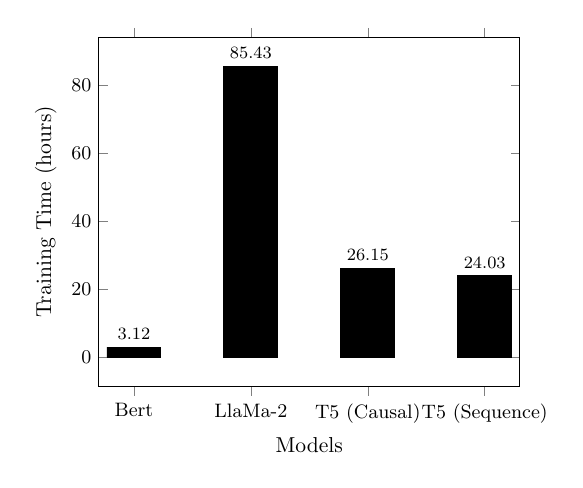
\begin{tikzpicture}[scale=0.78]
    \begin{axis}[
        ybar,                        
        enlargelimits=0.1,        
        xlabel={Models},     
        ylabel={Training Time (hours)},       
        symbolic x coords={Bert, LlaMa-2, T5 (Causal), T5 (Sequence)}, 
        xtick=data,                  
        ticklabel style={font=\small},
        nodes near coords,
        nodes near coords style={font=\footnotesize},
        bar width=25pt,          
        ymin=0                       
    ]
        \addplot  [fill=black] coordinates {(Bert, 3.12) (LlaMa-2, 85.43) (T5 (Causal), 26.15) (T5 (Sequence), 24.03)};
    \end{axis}
\end{tikzpicture}
	\caption{Health-Related Models Training Time} %specify caption
	\label{fig:HealthTime}
\end{figure}

\subsubsection{Training Time}

In Figure \ref{fig:HealthTime}, we present our model's training time. BERT trained faster than any other model, which took 3.12 hours. Both T5 models took over 24 hours to fine-tune. Lastly, LLaMa-2 took over three days to train. Based on these results, we can infer that models with fewer parameters train faster. BERT trained 27.4x faster than LLaMa-2.


\subsection{Misinformation Classification Results}
In this section, we present the misinformation classification results. However, we did not compare with the THS model because they did not train a model to classify misinformation.

\subsubsection{Precision}
\begin{table}[H]
	\centering
	\caption{Misinformation Precision Result}
	{\small
	\begin{tabular}{||c | c||} 
		\hline
		\textbf{Model} & \textbf{Result} \\  
		\hline
		BERT & 0.90  \\
		\hline
		LLaMa-2 & 0.98 \\ 
		\hline
		T5 (Causal) & 0.99 \\
		\hline
		T5 (Sequence) & 0.99 \\
		\hline
	\end{tabular}
	}
	\label{table:MisinformationPrecision}
\end{table}

Table \ref{table:MisinformationPrecision} shows the result for the precision metric for the misinformation classification. In this case, we focus on the misinformation
class because it is our project goal. Our best-performing models were both T5 models with a precision of 99\%. Nonetheless, all models had a score of at least 90\%.

\subsubsection{Recall}
\begin{table}[H]
	\centering
	\caption{Misinformation Recall Result}
	{\small
	\begin{tabular}{||c | c||} 
		\hline
		\textbf{Model} & \textbf{Result} \\ 
		\hline
		BERT & 0.94  \\
		\hline
		LLaMa-2 & 0.95 \\ 
		\hline
		T5 (Causal) & 0.92 \\
		\hline
		T5 (Sequence) & 0.85 \\
		\hline
	\end{tabular}
	}
	\label{table:MisinformationRecall}
\end{table}

Table \ref{table:MisinformationRecall} shows the recall metric's results for the misinformation classification. Here, the model with the best results was LLaMa-2,
with a performance of 95\%. While the lowest score was T5 (Sequence) ended with 85\% in the recall.

\subsubsection{F1}
\begin{table}[H]
	\centering
	\caption{Misinformation F1 Result}
	{\small
	\begin{tabular}{||c | c||} 
		\hline
		\textbf{Model} & \textbf{Result} \\  
		\hline
		BERT & 0.92  \\
		\hline
		LLaMa-2 & 0.97 \\ 
		\hline
		T5 (Causal) & 0.96 \\
		\hline
		T5 (Sequence) & 0.92 \\
		\hline
	\end{tabular}
	}
	\label{table:MisinformationF1}
\end{table}

Table \ref{table:MisinformationF1}  shows the result for the F1 metric for the misinformation classification. The results show that LLaMa-2 had the highest F1 with a 97\%.
However, all models had an F1 score of at least 90\%.

\subsubsection{Training Time}

\begin{figure}[H]
	\centering
	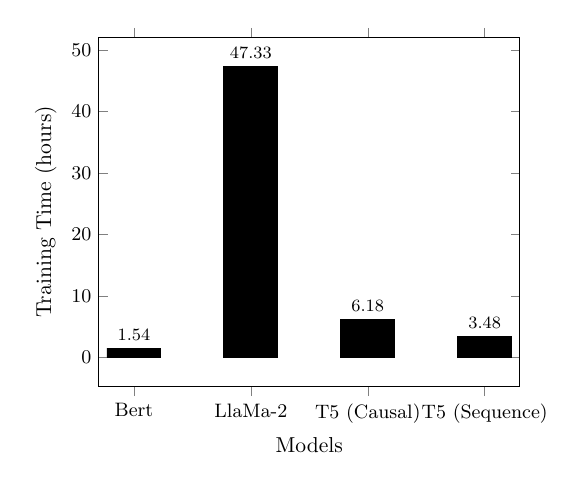
\begin{tikzpicture}[scale=0.78]
    \begin{axis}[
        ybar,                        
        enlargelimits=0.1,        
        xlabel={Models},     
        ylabel={Training Time (hours)},       
        symbolic x coords={Bert, LlaMa-2, T5 (Causal), T5 (Sequence)}, 
        xtick=data,                  
        ticklabel style={font=\small},
        nodes near coords,    
       	nodes near coords style={font=\footnotesize},
        bar width=25pt,          
        ymin=0                       
    ]
        \addplot  [fill=black] coordinates {(Bert, 1.54) (LlaMa-2, 47.33) (T5 (Causal), 6.18) (T5 (Sequence), 3.48)};
    \end{axis}
\end{tikzpicture}
	\caption{Misinformation Models Training Time} %specify caption
	\label{fig:MisinformationTime}
\end{figure}

In Figure \ref{fig:MisinformationTime}, we present the training time for the misinformation models. The model that trained the fastest was BERT, which took 1.54 hours. Next is T5 (Sequence) with 3.48 hours
and T5 (Causal) with 6.18 hours. Finally, LLaMa-2 took almost 2 days to train, 30.73x slower than BERT.

\subsection{BERTScore Result}

Our model BERTScores'  F1 is shown in Table \ref{table:BERTScore}. We calculate these values by taking the average score of the 71 texts classified as health-related and misinformation. The table shows that both models, had a 82\% F1 score. That means that the generated output are closely related but not exactly the same. 

\begin{table}[H]
	\centering
	\caption{BERTScore F1 Results}
	\begin{tabular}{||c | c||} 
		\hline
		\textbf{Model} & \textbf{Result} \\  
		\hline
		LLaMa-3.1 & 82\%  \\
		\hline
		GPT-3.5-turbo & 82\% \\ 		
		\hline
		\end{tabular}
	\label{table:BERTScore}
\end{table}

\subsection{Discussion}

The results present that most LLMs outperformed the THS model. We applied preprocessing techniques such as replacing links, mentions, and hashtags with special tokens.
The score metrics we used to evaluate the classification process were precision, recall, and F1. In our case, we want to focus on F1. In the health field, false negative should be
as low as possible. A false negative is missing a misinformation post that could pose a health risk to someone. However, we do not want a high number of false positive. Overclassifying 
texts as misinformation is also bad, because users might get skeptical of the veracity of the system. Additionally, the process of classification is slow when rebutting, that is why we need a balance.

Our model with the best result for the health-related classification (Table \ref{table:HealthF1}) was T5 (Causal), with a 90\% F1 score, while the THS model had 86\%. However, the trade-off
for this model is that the training is computationally expensive. T5 (Causal) labels are texts instead of numbers, they must be embedded, which requires more processing power. Also,
that model cannot have class weights because of the structure of the embedding. Additionally, the training time (Figure \ref{fig:HealthTime}) for T5 is more extensive
when compared to BERT, 8.4x. Now, BERT had a slightly lower result with 88\%. Nonetheless, when we factor in the training time and processing power, this model is more efficient.

The model with the highest F1 score for the misinformation classification (Table \ref{table:MisinformationF1}) was LLaMa-2 with 97\%. However, it requires high computational power and is
the model with the most extensive training time (Figure \ref{fig:MisinformationTime}). When compared to BERT, it takes 30.90x more time to train. However, LLaMa-2 outperform the
other models by a slight margin. 

For the BERTScore, our results shows that both models had an identical performance (Table \ref{table:BERTScore}). A possible reason is that the RAG process gives sufficient context to generate a
coherent response. However, both models have their trade-offs. To use GPT-3.5-turbo, we must pay OpenAI to request their API. On the other hand, LLaMa-3.1 runs with Ollama, and we need
sufficient memory to execute the model. The use case for each one depends on the user's hardware.

This paper focuses on social media posts, and we know that there are frequent changes in how users interact. Additionally, when new diseases are found or named, we must retrain the
models to find new patterns. Retraining can be costly if the model requires excessive resources and extensive training. Thus, we can say that BERT had overall results to help combat
health misinformation on social media. That model had an F1 score of 88\% in health and 92\% in misinformation classification, was the fastest and required the least amount of resources to train.




